% -----------------------------------------------
% Template for ISMIR 2010
% (based on earlier ISMIR templates)
% -----------------------------------------------

\documentclass{article}
\usepackage{ismir2012,amsmath,cite}
\usepackage{graphicx}
\usepackage{array}

% Title.
% ------
\title{AMA LAB3: HARMONIC AND TONAL ANALYSIS}

% Single address
% To use with only one author or several with the same address
% ---------------
%\oneauthor
% {Names should be omitted for double-blind reviewing}
% {Affiliations should be omitted for double-blind reviewing}

% Two addresses
% --------------
\twoauthors
  {Jakue L\'{o}pez Armend\'{a}riz} {Universitat Pompeu Fabra \\ Music Technology Group}
  {H\`{e}ctor Parra Rodr\'{i}guez} {Universitat Pompeu Fabra \\ Music Technology Group}

% Three addresses
% --------------
%\threeauthors
%  {First author} {Affiliation1 \\ {\tt author1@ismir.edu}}
%  {Second author} {\bf Retain these fake authors in\\\bf submission to preserve the formatting}
%  {Third author} {Affiliation3 \\ {\tt author3@ismir.edu}}

% Four addresses
% --------------
%\fourauthors
%  {First author} {Affiliation1 \\ {\tt author1@ismir.edu}}
%  {Second author}{Affiliation2 \\ {\tt author2@ismir.edu}}
%  {Third author} {Affiliation3 \\ {\tt author3@ismir.edu}}
%  {Fourth author} {Affiliation4 \\ {\tt author4@ismir.edu}}

\begin{document}
%
\maketitle
%
\begin{abstract}
A simple key estimation system of polyphonic music signals is presented.
%The chroma features are computed to accomplish such task.
%First, both methods are individually studied to find their strong and weak characteristics.
%Finally, a mixing method for both strategies is proposed. This mixing method is able
%to balance the weight of each strategy in order to improve the results for each
%analyzed phrase.
\end{abstract}
%
\section{Chroma Feature Extraction}\label{sec:chroma}
Chroma features are an interesting and powerful representation for music audio in which the entire spectrum is projected onto a certain number of bins, e.g., 12 bins will represent the 12 distinct semitones (or chroma) of the musical octave. Traditionally, this task is approached as a polyphonic transcription to identify individual notes \cite{Fujishima:1999}. When these musical notes are exactly one octave apart from each other they are perceived similarly. Thus, knowing the distribution of chroma, even without knowing the absolute frequency, can give us meaningful musical information about the audio. It may also provide information about musical similarity that is not evident in the original spectrum. In the following section we will present and discuss three different approaches for chroma feature extraction. For this, we have selected the piano melody number 7 (in A\# Major) from the MIREX'05 key test dataset.

\subsection{Ellis Method}\label{subsec:chroma_ellis} %J
This package developed by Ellis, D.\footnote{http://www.ee.columbia.edu/~dpwe/resources/matlab/chroma-ansyn/} includes different ways to calculate chroma features. It also provides a routine that resynthesizes audio with the chromatic content defined by the features. In our case, we will use the {\it chromagram\_IF} function that obtains the features in the following way:

First, a pitch tracking based on instantaneous frequency is performed. Second, it searches for plateaus in the instantaneous frequencies over 2 KHz and smaller than a certain threshold. Third, it figures out the best tuning alignment and adjusts them to align better with the chroma. As a last step, to obtain the final chroma features, it quantizes and maps the instantaneous frequency pitches into chroma bins. In \figref{fig:chroma07ellis} we can observe the chroma features for each analyzed frame of the sound. In contrast, an average of the features can be observed in \figref{fig:averagechroma07ellis}.

\begin{figure}
 \centerline{\framebox{
 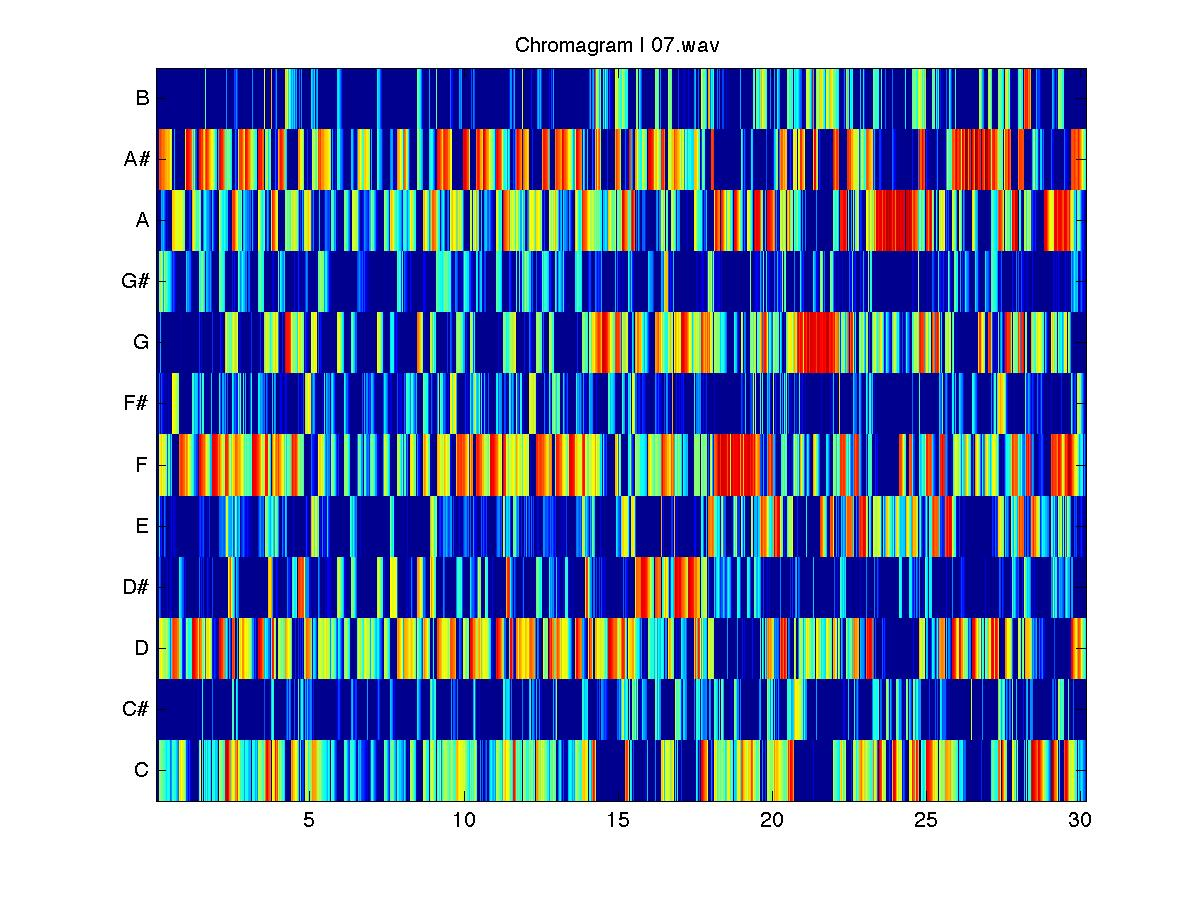
\includegraphics[width=\columnwidth]{figures/ellis/Chromagram_07_ellis.jpg}}}
 \caption{Instantaneous chroma features (Ellis, D.) of the melody number 7 (in A\# Major) from the MIREX'05 key test set.}
 \label{fig:chroma07ellis}
\end{figure}

\begin{figure}
 \centerline{\framebox{
 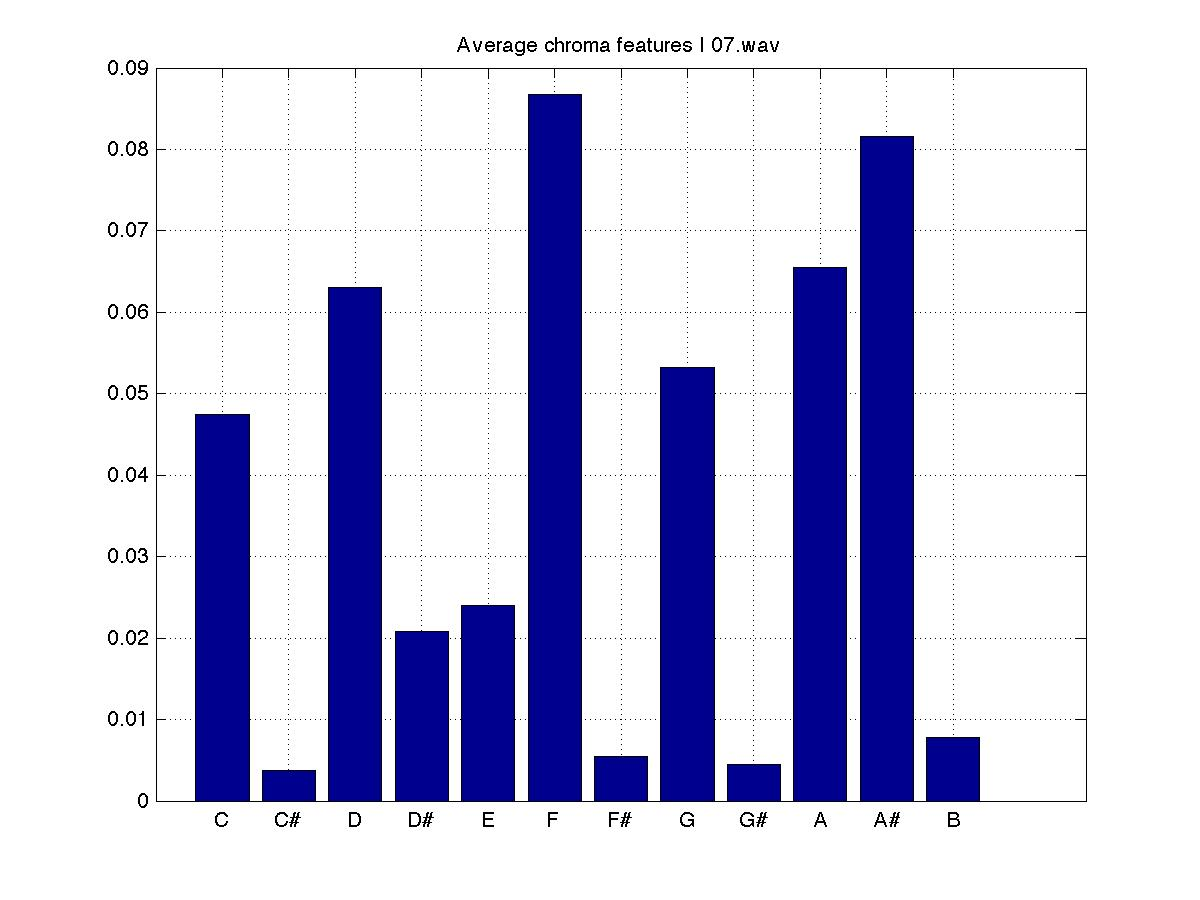
\includegraphics[width=\columnwidth]{figures/ellis/InstantChroma_07_ellis.jpg}}}
 \caption{Average chroma features (Ellis, D.) of the melody number 7 (in A\# Major) from the MIREX'05 key test set.}
 \label{fig:averagechroma07ellis}
\end{figure}

Finally, the resynthesis tool turns the features into an audio signal. It simply uses the 12 chroma values to modulate 12 sinusoids that are tuned to cover one octave. As the octave would be arbitrary, each chroma value modulates an ensemble of sinusoids, with frequencies related by a power of two, that share the same chroma. A smooth rolloff to these sinusoids at high and low extremes of the spectrum provides a chroma without a clear sense of octave. These tones are known as {\it Shepard Tones}. The synthesized spectrogram can be observed in \figref{fig:resynth07ellis}. The synthesized audio is far away from the original sound. The melody is preserved but the timbre is notably changed. 

\begin{figure}
 \centerline{\framebox{
 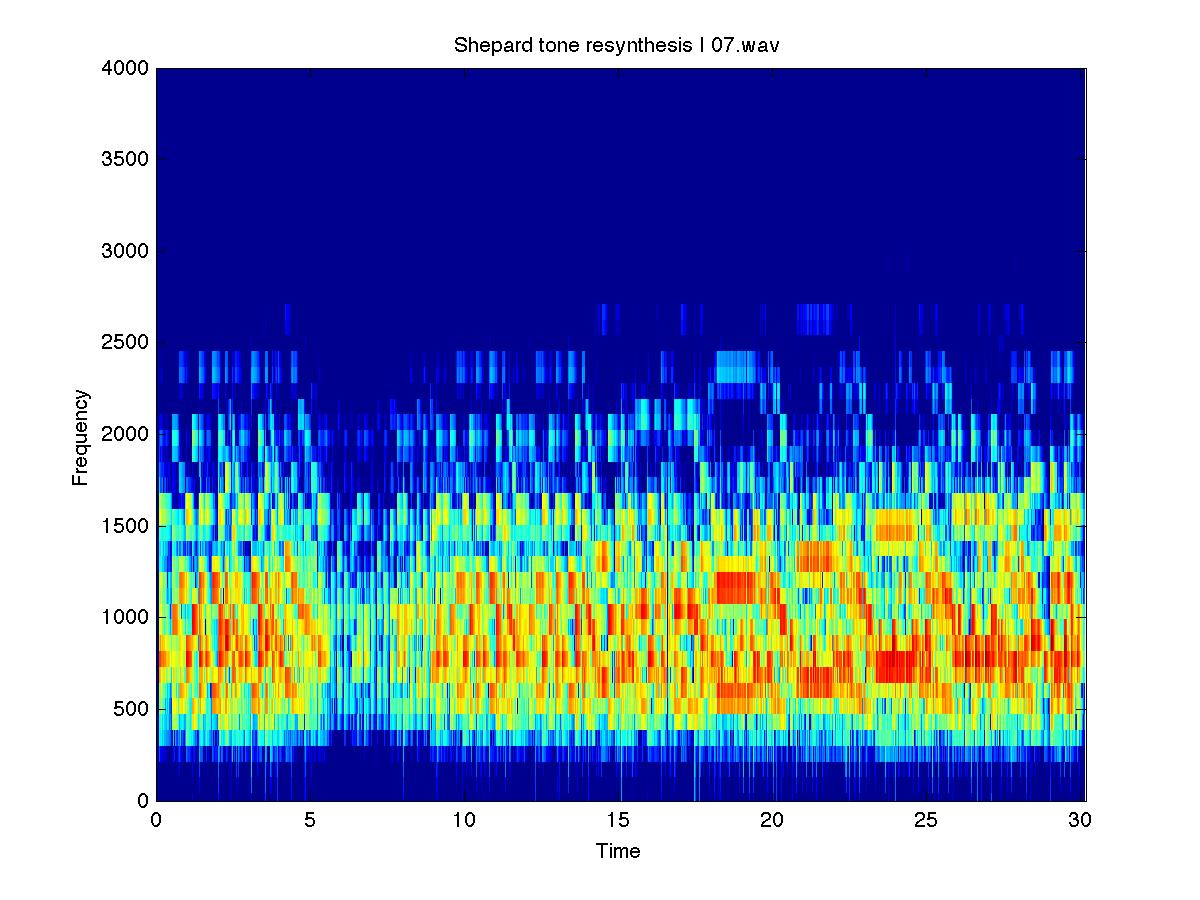
\includegraphics[width=\columnwidth]{figures/ellis/resynth_07.jpg}}}
 \caption{Resynthesized audio spectrum from chroma features (Ellis, D.) of the melody number 7 (in A\# Major) from the MIREX'05 key test set.}
 \label{fig:resynth07ellis}
\end{figure}

\subsection{Chroma Toolbox 2.0}\label{subsec:chroma_toolbox} %H
The Chroma Toolbox\cite{Author:Muller} contains MATLAB implementations\footnote{http://www.mpi-inf.mpg.de/resources/MIR/chromatoolbox/} for the extraction of pitch and various chroma-like features and have been developed by Meinard M{\"u}ller and Sebastian Ewert.
In a first step, the audio signal is decomposed into 88 frequency bands with center frequencies corresponding to pitches A0 to C8. This decomposition is realized by a multirate filter bank of elliptic filters. For each subband the short-time mean-square power (STMSP) is computed. This process allows the measurement of the local energy content of each pitch subband, thus indicating the presence of certain musical notes.
From this point, \textbf{CP} (Chroma Pitch), that is a chroma-based descriptor, is derived by summing up pitch subbands that correspond to the same pitch class (e.g. chroma A is the sum of STMSPs of A0, A1, ..., A7). Furthermore, to account for the logarithmic sensation of sound by the human auditory system it can be applied a logarithmic compression of the pitch features before the chroma computation; the resulting features are referred to as \textbf{CLP} features.
By considering short-time statistics over energy distributions within the chroma bands, \textbf{CENS} (Chroma Energy Normalized Statistics) features\cite{Author:Muller2} can be extracted. These strongly correlate to the short-time harmonic content of the underlying audio signal and absorb variations of properties such as dynamics, timbre, articulation, execution of note groups, and temporal micro-deviations.
Finally, to boost the degree of timbre invariance, \textbf{CRP} (Chroma DCT-Reduced log Pitch) features can be used . The extraction consists on using a nonlinear pitch scale and applying a DCT (Discrete Cosine Transform) on the logarithmized pitch representation to obtain pitch-frequency cepstral coefficients (PFCCs). Then, only the upper coefficients are kept (since low coefficients mostly contain timbre information), the inverse DCT is used and eventually the resulting pitch vectors are projected onto 12-dimensional chroma vectors.
\figref{fig:chroma07crp} and \figref{fig:averagechroma07crp} show the over time (in frame per frame basis) and averaged CRP features, respectively.

\begin{figure}
 \centerline{\framebox{
 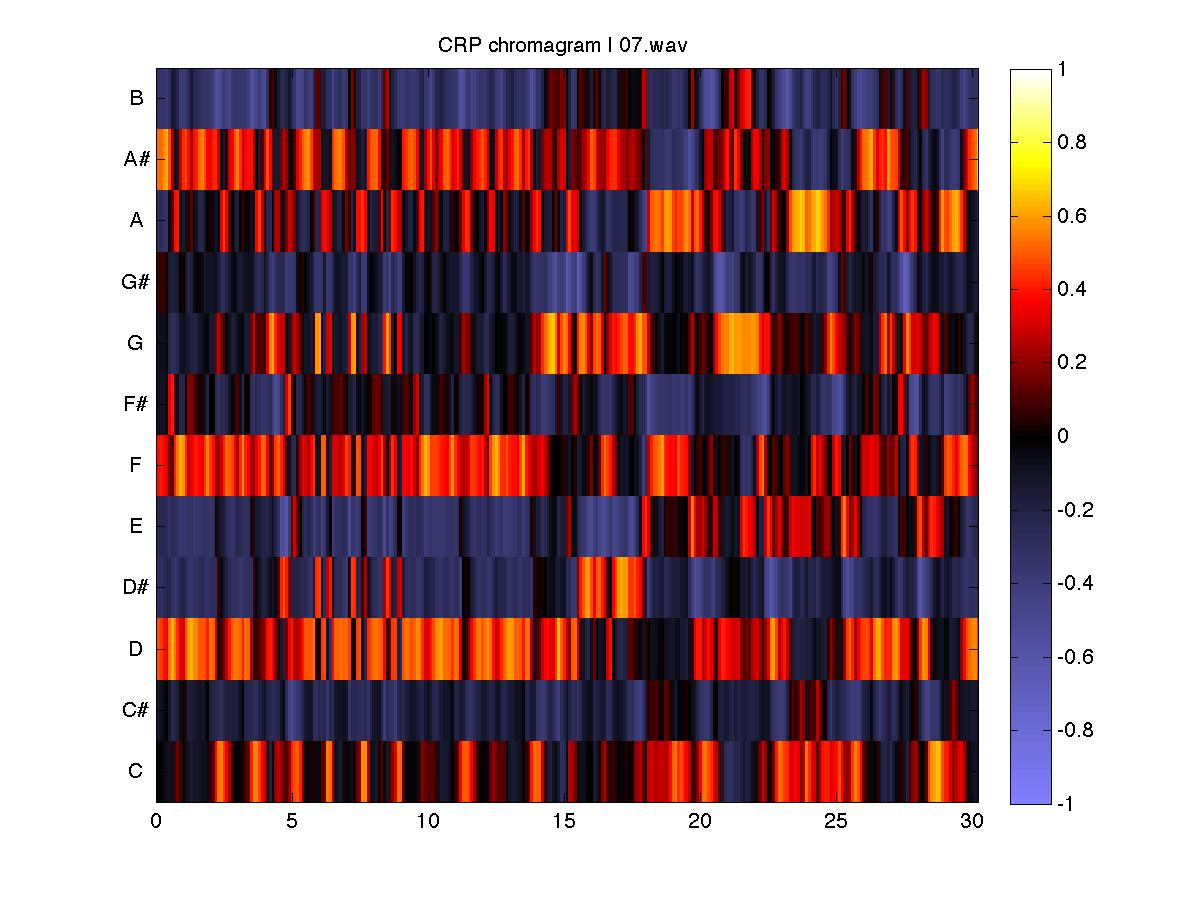
\includegraphics[width=\columnwidth]{figures/chroma_toolbox/Chromagram_07_toolbox.jpg}}}
 \caption{Instantaneous chroma features (CRP) of the melody number 7 (in A\# Major) from the MIREX'05 key test set.}
 \label{fig:chroma07crp}
\end{figure}

\begin{figure}
 \centerline{\framebox{
 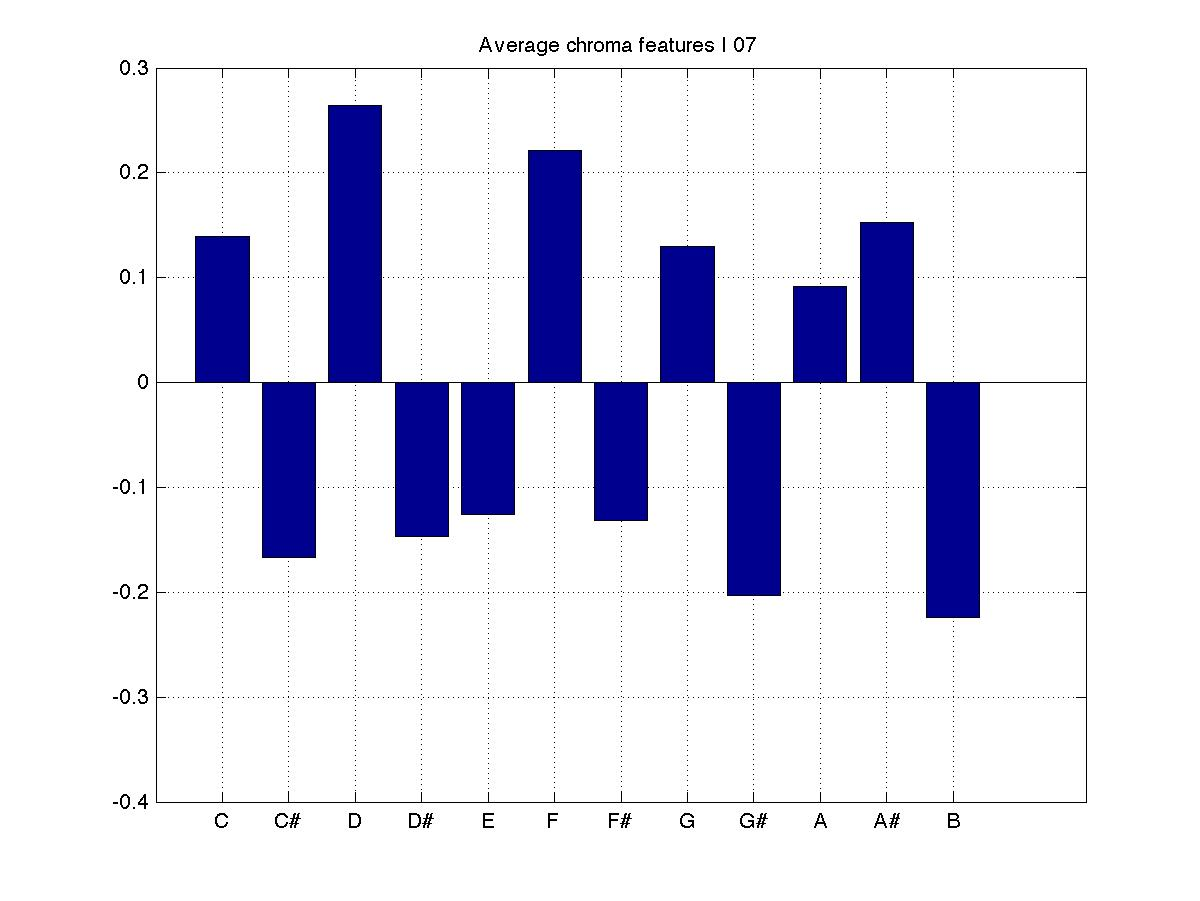
\includegraphics[width=\columnwidth]{figures/chroma_toolbox/InstantChroma_07_toolbox.jpg}}}
 \caption{Average chroma features (CRP) of the melody number 7 (in A\# Major) from the MIREX'05 key test set.}
 \label{fig:averagechroma07crp}
\end{figure}

\subsection{Harmonic Pitch Class Profile}\label{subsec:chroma_hpcp} %J

This system, developed by G{\'o}mez, E. and Bonada, J, allows an automatic tonal description of audio. For this task, we have used the vamp plug-in implementation\footnote{http://mtg.upf.edu/technologies/hpcp/}. Here, the extracted features are called {\it Harmonic Pitch Class Profile} and they represent the relative intensity of each bin in one octave (considering an equal-tempered scale tuned to the reference frequency). The computation is performed by taking the peaks of the magnitude spectrum in a certain frequency band. This band is considered to contain the most significant frequencies that represent the harmonic properties. In addition, by introducing a weight, the different tunings and inharmonicity are taken into account. As a last step, for each frame the HPCP vector is normalized to discard energy information\cite{gomez05}. \figref{fig:chroma07hpcp} and \figref{fig:averagechroma07hpcp} show the HPCP features for each analyzed frame and for the averaged values, respectively.

\begin{figure}
 \centerline{\framebox{
 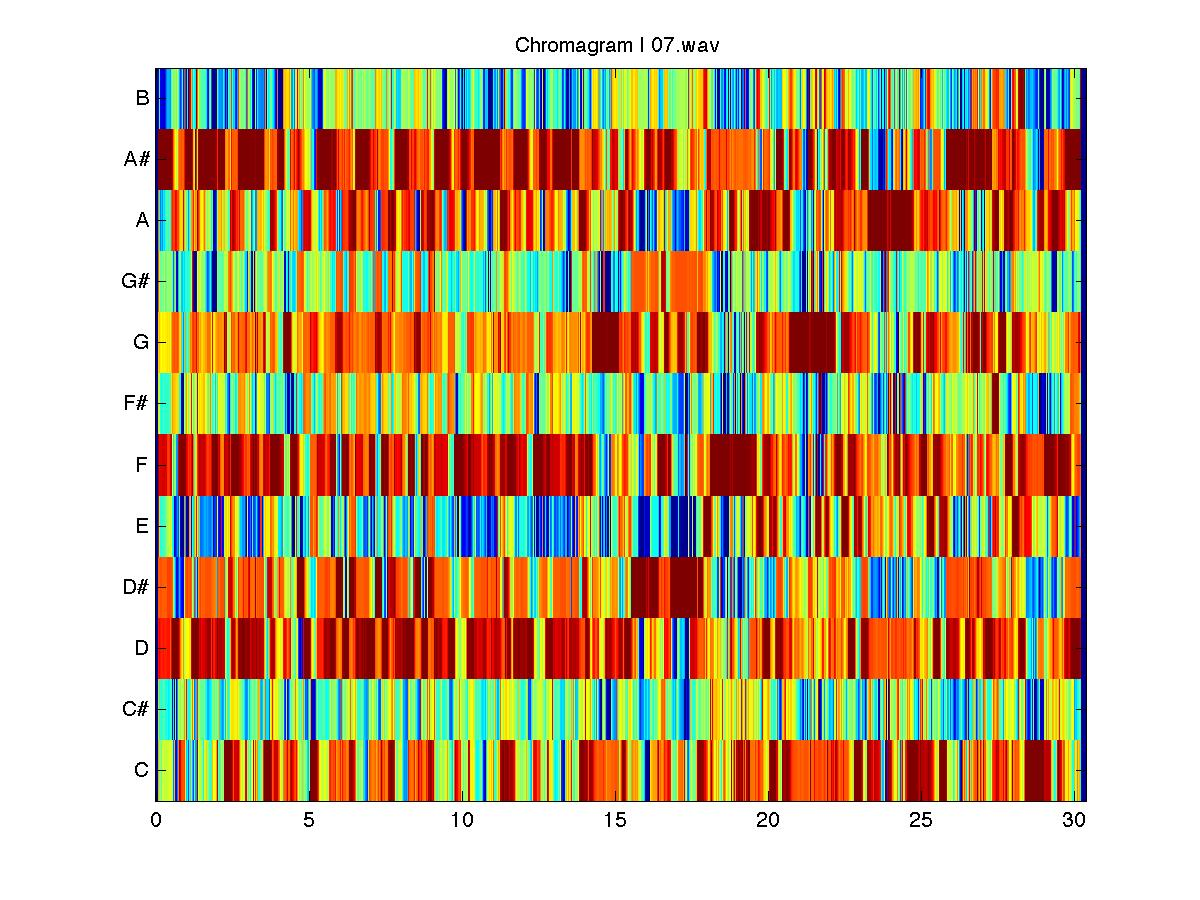
\includegraphics[width=\columnwidth]{figures/hpcp/Chromagram_07_hpcp.jpg}}}
 \caption{Instantaneous chroma features (HPCP) of the melody number 7 (in A\# Major) from the MIREX'05 key test set.}
 \label{fig:chroma07hpcp}
\end{figure}

\begin{figure}
 \centerline{\framebox{
 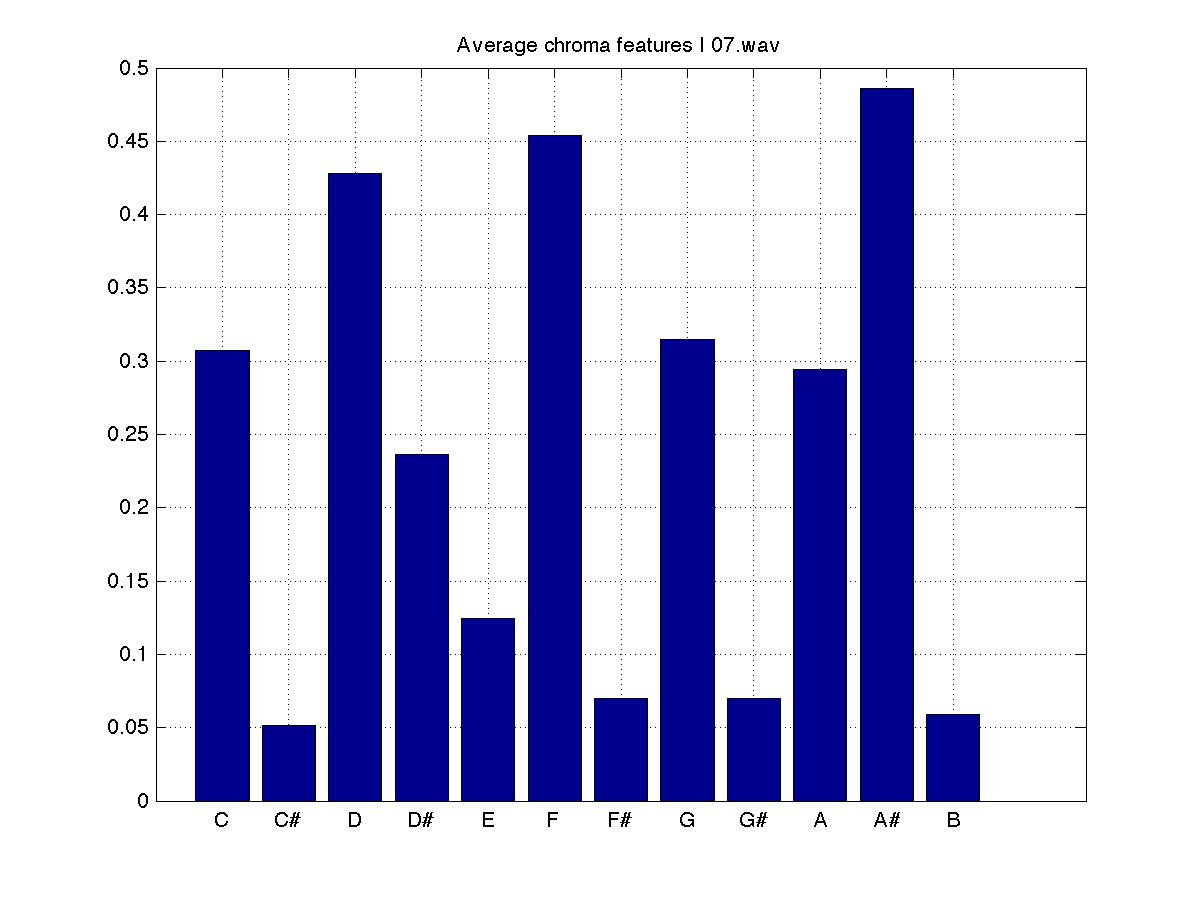
\includegraphics[width=\columnwidth]{figures/hpcp/InstantChroma_07_hpcp.jpg}}}
 \caption{Average chroma features (HPCP) of the melody number 7 (in A\# Major) from the MIREX'05 key test set.}
 \label{fig:averagechroma07hpcp}
\end{figure}

\subsection{Observations} %J & H review

The selected piano melody (07.wav) from the MIREX'05 key test set is tuned to a A\# major scale. This scale consists of the pitches A\#, C, D, D\#, F, G, and A. Both methods of Ellis and Chroma Toolbox give almost correct results, except for D\# pitch, where both fail by not giving a high value for it. HPCP seems to perform better by giving all the pitch values correctly, D\# included. Moreover, all of them have some weight at pitch E (not in the scale), probably a consequence of the strong presence of the 3rd major (D), whose perfect 5th (corresponds to the third harmonic) is an A (also very present), whose perfect fifth is an E. This argumentation gives some clues why weights of each note on a key chroma do not always coincide with their theoretical importance in the scale.

\section{Key Estimation} 
\subsection{Global Chroma Vector} %H
Although scores or pieces have a general key, the normally modulate (change key) along themselves, thus, the most exhaustive way to define the key should be the tonal mode used in short excerpts of a whole piece. Our algorithm takes a simplified approach and assumes a constant key when analyzing pieces, so a final chroma vector for the key is computed by averaging chroma frame values for the entire piece. This is an important fact to not use this method with too long pieces. In classical music, as a general rule of thumb, a minute starts to be too much. In fact, the pieces used in our evaluation (Section \ref{sec:eval}) have an average length of 30 seconds.

\subsection{Pattern Matching}	%J
% FIX: This is written in future. Use past (sometimes present) in reports
For each of the chroma vectors we have extracted, we will compute a pattern matching algorithm with different key or tonal profiles. These key profiles represent the knowledge of musical keys by the relative importance of the tones in the chromatic scale. We will obtain the key of the musical segment by relaying on the idea that the pitch class distribution of the notes in a piece of music could reveal its tonality. Simply by calculating the correlation of the distribution with each of the 12 major and 12 minor profiles, and predicting the highest correlated key. % FIX: this last sentence has no main verb

We have selected four different key profiles for their comparison: First, Krumhansl and Kessler\cite{Author:Krumhansl} suggested that tonal hierarchies could be represented by probe tone profiles. They assume that a pattern matching mechanism between the tonal hierarchies and the distribution of pitches in a musical piece models the way listeners arrive at a sense of key. Second, Temperley \cite{Author:Temperley} proposed an extension of this model. Third, the Diatonic profile can be viewed as a flat profile which responds to presence or absence of pitches but lacks sensitivity of the relative importance of pitches. Fourth, a composite model based in the combination of Temperley's profile with the Diatonic profile proposed in \cite{Author:Izmirli}.

\tabref{tab:keyprofs} shows the key profiles values for the four approaches.



%                'composite': {
%                    'major': [5.0, 0.0, 3.5, 0.0, 4.5, 4.0, 0.0, 4.5, 0.0, 3.5, 0.0, 4.0],
%                    'minor': [5.0, 0.0, 3.5, 4.5, 0.0, 4.0, 0.0, 4.5, 3.5, 0.0, 0.0, 4.0]}}
%                        

\begin{table}
 \begin{center}
 \begin{tabular}{|l|c|c|c|c|c|c|c|c|}
   \hline
  C			&	kM		&	km		&	tM		&	tm		&	dM	 &	dm	& 	cM		&	cm		\\
  \hline
  	0		&	6.35	&	6.33	&	5.00	&	5.00	&	1 	 &	1	&	5.00	&	5.00	\\
  	1		&	2.23	&	2.68	&	2.00	&	2.00	&	0	 &	0	&	0.00	&	0.00	\\
  	2		&	3.48	&	3.52	&	3.50	&	3.50	&	1	 &	1	&	3.50	&	3.50	\\  
  	3		&	2.33	&	5.38	&	2.00	&	4.50	&	0	 &	1	&	0.00	&	4.50	\\  
  	4		&	4.38	&	2.6		&	4.50	&	2.00	&	1	 &	0	&	4.50	&	0.00	\\
  	5		&	4.09	&	3.53	&	4.00	&	4.00	&	1	 &	1	&	4.00	&	4.00	\\
  	6		&	2.52	&	2.54	&	2.00	&	2.00	&	0	 &	0	&	0.00	&	0.00	\\  
  	7		&	5.19	&	4.75	&	4.50	&	4.50	&	1	 &	1	&	4.50	&	4.50	\\ 
  	8		&	2.39	&	3.98	&	2.00	&	3.50	&	0	 &	1	&	0.00	&	3.50	\\
  	9		&	3.66	&	2.69	&	3.50	&	2.00	&	1	 &	0	&	0.00	&	0.00	\\
  	10		&	2.29	&	3.34	&	1.50	&	1.50	&	0	 &	0	&	0.00	&	0.00	\\  
  	11		&	2.88	&	3.17	&	4.00	&	4.00	&	1	 &	1	&	4.00	&	4.00	\\ 	
  \hline
 \end{tabular}
\end{center}
 \caption{Krumhansl and Kessler, Diatonic, Temperley�s and composite pitch distribution profiles. C: Chroma, kM: Krumhansl and Kessler Major, km: Krumhansl and Kessler's minor, tM: Temperley major, tm: Temperley minor, dM: Diatonic major, dm: Diatonic harmonic minor, cM: composite major and cm: composite minor.}
 \label{tab:keyprofs}
\end{table}

Two matching methods are compared, correlation and weighted sum. % This has to be explained?
%
%compute correlation with key profiles
%	key profiles
%	table -> key profiles  
%	correlation formula?

\section{Evaluation and Results}\label{sec:eval} %H

For the evaluation we used the MIREX 2005 key test set: a collection of 96 classical music pieces synthesized directly from its midi score. These pieces have a short duration (around 30 seconds) and its ground truth consists on a single key (e.g. G\# major or Bb minor), so it fits with the requirements of our algorithm that supposes a unique key per piece. Moreover, this dataset only contains major and minor modes for each of the 12 possible semitones from the diatonic scale tuned to a 440Hz reference.
The evaluation method used was precision. We consider that the result is correct if both the key tonic and the mode are matched, but it will be incorrect even if only one of them is matched.
On the other hand, we used the three methods presented in Section \ref{sec:chroma} (they are actually six since we used the four possibilities that the Chroma Toolbox offers, explained in Section \ref{subsec:chroma_toolbox}) for extracting chroma features.
Moreover, although two pattern matching strategies were used, the results and tables presented correspond to the correlation results since the weighted sum strategy always performed worst.

For our results our first study consited in computing the precision of each chroma features against the four pitch distribution profiles in Table \ref{tab:keyprofs}. This is shown in Table \ref{tab:precision}, were we can see the best result was obtained was \textbf{71.88\%} using HPCP features against Temperley pitch profile. In this case, the weighted sum strategy gave the same best result also for HPCP and Temperley.
Our second study tried to improve our previous results by creating our own adapted pitch distribution profiles. First, we extracted those profiles from the same database we were analyzing (this is called overfitting, since our tools are adapted exclusively for the data we evaluate). This process consisted on aligning the chroma of each piece with the same mode (e.g. B major has to be translated two semitones downwards to be aligned with C major) and then averaging all these chromas separated for every mode, in our case only major and minor. These pitch distribution profiles are shown in Table \ref{tab:extracted_profiles_M} for major mode and Table \ref{tab:extracted_profiles_m} for minor mode. Finally, we computed precision with these profiles following the same process as in our first experiment; results are shown in Table \ref{tab:precision_extracted}. This time a maximum precision of \textbf{93.75\%} was achieved using CENS features and the pitch profile extracted using CLP features. In the case of using the weigthed sum strategy a 89.58\% was obtained using CENS features with the pitch profile extracted using CP features.


\section{Conclusions} %J

%shitty results
%
%Chroma:
%	hpcp > toolbox > ellis
%
%Pitch profiles:
%	temperley > composite
%	diatonic equal for all
%	krumhansl good for hpcp 
%
%Important to have a good compromise between pitch profiles an chroma extraction. 
%Choose the proper pitch profiles according to the selected chroma extraction method.

\subsection{Future work}
other strategies for pattern matching different to correlation can be used. For example: Nearest neighbor, weighted sum
create our own pitch profiles to improve the results with the used database
use more bins (more than 12) to have more precision -> create corresponding pitch profiles too

\section{Appendix}

To facilitate the reproducibility of this report we provide open access to its implementation code\footnote{https://github.com/hector/ama/tree/732c4322a56a5217a58e977f83a962bc47b120e5} % update link

%\section{Footnote}
%
%Indicate footnotes with a number in the text.\footnote{This is a footnote.}
%Use 8pt type for footnotes. Place the footnotes at the bottom of the page on which they appear.
%Precede the footnote with a 0.5pt horizontal rule.
%
%\subsection{Figures, Tables and Captions}
%
%All artwork must be centered, neat, clean, and legible.
%All lines should be very dark for purposes of reproduction and art work should not be hand-drawn.
%The proceedings are not in color, and therefore all figures must make sense in black-and-white form.
%Figure and table numbers and captions always appear below the figure.
%Leave 1 line space between the figure or table and the caption.
%Each figure or table is numbered consecutively. Captions should be Times 10pt.
%Place tables/figures in text as close to the reference as possible.
%References to tables and figures should be capitalized, for example:
%see \figref{fig:example} and \tabref{tab:example}.
%Figures and tables may extend across both columns to a maximum width of 17.2cm.
%
%\begin{table}
% \begin{center}
% \begin{tabular}{|l|l|}
%  \hline
%  String value & Numeric value \\
%  \hline
%  Hello ISMIR  & 2012 \\
%  \hline
% \end{tabular}
%\end{center}
% \caption{Table captions should be placed below the table.}
% \label{tab:example}
%\end{table}
%
%\begin{figure}
% \centerline{\framebox{
% \includegraphics[width=\columnwidth]{figure.png}}}
% \caption{Figure captions should be placed below the figure.}
% \label{fig:example}
%\end{figure}
%
%\section{Equations}
%
%Equations should be placed on separated lines and numbered.
%The number should be on the right side, in parentheses.
%
%\begin{equation}
%E=mc^{2}
%\end{equation}
%
%\section{Citations}
%
%All bibliographical references should be listed at the end,
%inside a section named ``REFERENCES,'' numbered and in alphabetical order.
%Also, all references listed should be cited in the text.
%When referring to a document, type the numbering square brackets
%\cite{Author:00} or \cite{Author:00,Someone:10,Someone:04}.
%
\begin{thebibliography}{citations}

\bibitem {Fujishima:1999}
Fujishima, T:
``Realtime chord recognition of musical sound: A system using common lisp music,''  
{\it Proc ICMC 1999}, 
Vol. ~9, No.~6, pp.~464--467, 1999.

\bibitem {gomez05}
G{\'o}mez, E. and Bonada, J:
``Tonality visualization of polyphonic audio,''
2005.

\bibitem {Author:Muller}
Meinard M{\"u}ller and Sebastian Ewert:
``{C}hroma {T}oolbox: {MATLAB} implementations for extracting variants of chroma-based audio features,''
{\it Proceedings of the 12th International Conference on Music Information Retrieval ({ISMIR})}, 2011.

\bibitem {Author:Muller2}
Meinard M{\"u}ller, Frank Kurth, and Michael Clausen:
``Audio Matching via Chroma-Based Statistical Features,''
{\it Proceedings of the 6th International Conference on Music Information Retrieval ({ISMIR})}, pp.~288--295, 2005.

\bibitem {Author:Krumhansl}
Carol L. Krumhansl and E. J. Kessler: 
``Tracing the dynamic changes in perceived tonal organisation in a spatial representation of musical keys,''
{it\ Psychological Review}, 89:334�368, 1982.

\bibitem {Author:Temperley}
Temperley, D. 
``What�s Key for Key? The Krumhansl-Schmuckler Key-Finding Algorithm Reconsidered,''
{\it Music Perception}, 17(1):65�100, 1999.

\bibitem {Author:Izmirli}
\"O. Izmirli:
``An algorithm for audio key finding'' 
{\it in Abstract of the 1st Annual Music Information Retrieval Evaluation eXchange (MIREX'05)}, London, UK, 2005.

%E. Author:
%``The Title of the Conference Paper,''
%{\it Proceedings of the International Symposium
%on Music Information Retrieval}, pp.~000--111, 2000.
%
%\bibitem{Someone:10}
%A. Someone, B. Someone, and C. Someone:
%``The Title of the Journal Paper,''
%{\it Journal of New Music Research},
%Vol.~A, No.~B, pp.~111--222, 2010.

%\bibitem{Someone:04} X. Someone and Y. Someone: {\it Title of the Book},
%    Editorial Acme, Porto, 2012.
%
\end{thebibliography}

\bibliography{ismir2012template}

\begin{table}
 \begin{center}
 \renewcommand{\arraystretch}{1.3}
 \begin{tabular}{|l|c|c|c|c!{\vrule width 1pt}c|}
	\hline
				&	Comp.	&	Diat.	&	Krum.	&	\bf{Temp.}	& 	\it{Mean}	\\
	\hline
  	Ellis		&	46.88	&	36.46	&	25.00	&	48.00		&	39.09		\\
  	\bf{HPCP}	&	63.54	&	53.12	&	64.58	&	\bf{71.88}	&	\it{63.28}	\\
  	CENS			&	62.50	&	53.13	&	63.54	&	66.67		&	61.46		\\
  	CLP			&	59.38	&	42.71	&	50.00	&	59.38		&	52.87		\\
  	CP			&	61.46	&	51.04	&	53.13	&	65.63		&	57.82		\\
  	CRP			&	48.96	&	39.59	&	33.33	&	52.08		&	43.49		\\
  	\noalign{\hrule height 1pt}
  	\it{Mean}	&	57.12	&	45.91	&	48.26	&	\it{60.61}	&	\bf{53.00}	\\  	
 	\hline
 \end{tabular}
\end{center}
 \caption{Precision (in percentage) for each chroma features (rows) vs. pitch distribution profiles (columns) computed for the MIREX05 key test set. Abbreviations stand for Comp.: composite, Diat.: diatonic, Krum.: krumhansl, Temp.: temperley}
 \label{tab:precision}
\end{table}

\begin{table}
 \begin{center}
 \begin{tabular}{|l|c|c|c|c|c|c!{\vrule width 1pt}c|}
   \hline
				&	Ellis	&	HPCP		&	CENS		&	\bf{CLP} 	&	CP		&	CRP		&	Mean			\\
  \hline
  	Ellis		&	43.75	&	56.25	&	68.75	&	72.92		&	67.71	&	69.79	&	63.20		\\
  	HPCP			&	42.71	&	82.29	&	90.63	&	89.58		&	91.67	&	78.13	&	79.17		\\
  	\bf{CENS}	&	48.96	&	83.33	&	91.67	&	\bf{93.75}	&	91.66	&	89.58	&	\it{83.16}	\\
  	CLP			&	59.38	&	76.04	&	86.46	&	89.58		&	88.54	&	83.33	&	80.56		\\
  	CP			&	48.96	&	79.17	&	87.50	&	91.67		&	87.5		&	85.42	&	80.07		\\
  	CRP			&	45.83	&	51.04	&	69.79	&	78.13		&	68.75	&	84.38	&	66.32		\\
  	\noalign{\hrule height 1pt}
  	Mean			&	48.27	&	71.41	&	82.47	&	\it{85.94}	&	82.64	&	81.77	&	\bf{75.42}	\\
  \hline
 \end{tabular}
\end{center}
 \caption{Precision (in percentage) for each chroma features (rows) vs. pitch distribution profiles (columns) extracted from the MIREX05 key test set using this same chroma features. Results computed against the same MIREX05 key set}
 \label{tab:precision_extracted}
\end{table}

\begin{table}
 \begin{center}
 \begin{tabular}{|l|c|c|c|c|c|c|c|c|}
   \hline
  			&	Ellis	&	HPCP		&	CENS		&	CLP		&	CP		&	CRP		\\
  \hline
  	0		&	0.80		&	0.98		&	0.92		&	0.94		&	0.93		&	0.68		\\
  	1		&	0.12		&	0.16		&	0.06		&	0.24		&	0.11		&	-0.99	\\
  	2		&	0.72		&	0.71		&	0.64		&	0.71		&	0.65 	&	0.61		\\
  	3		&	0.11		&	0.16		&	0.07		&	0.22		&	0.12 	&	-0.53	\\
  	4		&	0.83		&	0.75		&	0.76		&	0.79		&	0.76  	&	0.77		\\
  	5		&	0.34		&	0.54		&	0.42		&	0.48		&	0.42  	&	-0.35	\\
  	6		&	0.28		&	0.28		&	0.18		&	0.38		&	0.23  	&	-0.63	\\
  	7		&	1.00		&	1.00		&	1.00		&	1.00		&	1.00  	&	1.00		\\
  	8		&	0.11		&	0.18		&	0.07		&	0.24		&	0.12  	&	-0.62	\\
  	9		&	0.56		&	0.60		&	0.50		&	0.59		&	0.52  	&	0.49		\\
  	10		&	0.11		&	0.20		&	0.07		&	0.22		&	0.11  	&	-0.68	\\
  	11		&	0.63		&	0.57		&	0.54		&	0.66		&	0.55  	&	0.26		\\
  \hline
 \end{tabular}
\end{center}
 \caption{Normalized pitch distribution profiles for a major scale extracted extracted from the MIREX05 key test set using this same chroma features (indicated in the columns)}
 \label{tab:extracted_profiles_M}
\end{table}

\begin{table}
 \begin{center}
 \begin{tabular}{|l|c|c|c|c|c|c|c|c|}
   \hline
  			&	Ellis	&	HPCP		&	CENS		&	CLP		&	CP		&	CRP		\\
  \hline
  	0		&	0.77		&	0.95		&	0.88		&	0.89		&	0.87		&	0.70		\\
  	1		&	0.12		&	0.19		&	0.07		&	0.20		&	0.11		&	-1.00	\\
  	2		&	0.66		&	0.69		&	0.67		&	0.73		&	0.68 	&	0.37		\\
  	3		&	0.58		&	0.68		&	0.66		&	0.67		&	0.65 	&	0.40		\\
  	4		&	0.18		&	0.25		&	0.10		&	0.25		&	0.15  	&	-0.37	\\
  	5		&	0.50		&	0.64		&	0.51		&	0.55		&	0.53  	&	0.16		\\
  	6		&	0.20		&	0.25		&	0.17		&	0.31		&	0.21  	&	-0.53	\\
  	7		&	1.00		&	1.00		&	1.00		&	1.00		&	1.00  	&	0.88		\\
  	8		&	0.31		&	0.44		&	0.35		&	0.40		&	0.36  	&	-0.44	\\
  	9		&	0.32		&	0.33		&	0.23		&	0.37		&	0.27  	&	-0.15	\\
  	10		&	0.49		&	0.54		&	0.40		&	0.50		&	0.43  	&	0.17		\\
  	11		&	0.27		&	0.37		&	0.30		&	0.40		&	0.32  	&	-0.16	\\
  \hline
 \end{tabular}
\end{center}
 \caption{Normalized pitch distribution profiles for a minor scale extracted extracted from the MIREX05 key test set using this same chroma features (indicated in the columns)}
 \label{tab:extracted_profiles_m}
\end{table}

\end{document}
